The user begins by using Karma's existing capability to capture the artists in the first CSV file as crm:E21\_Person from the CIDOC CRM ontology in an R2RML mapping shown in Figure~\ref{fig:simple-model-screenshot}.  
Karma can use this mapping to generate RDF. 
Karma can also compare it to the other mappings loaded in the Model Manager to discover new related sources that can be used to augment the data.
\begin{figure*}[bh]
\centering
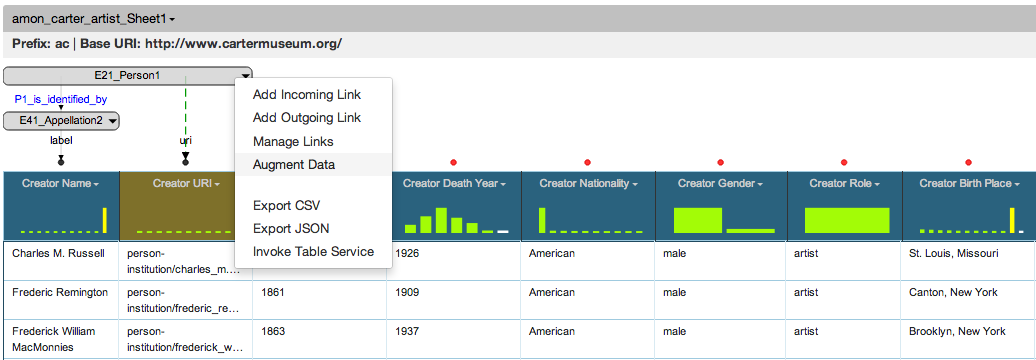
\includegraphics[width=4.8in]{images/4-simple-model.png}
\vspace{-20pt}
\caption{A Karma user creates an R2RML mapping for a CSV file of a museum's artists' biographical records and clicks 'Augment Data' to discover new data sources}
\vspace{-21pt}
\label{fig:simple-model-screenshot}
\end{figure*}